\documentclass{article}
\usepackage{graphicx}
\usepackage{amsmath}
\usepackage{float} % For float placement

\title{Pneumothorax Detection and Classification in Chest X-rays}
\author{yaser zaidan}
\date{25/9/2024}

\begin{document}

\maketitle

\section*{Introduction}
Pneumothorax is a critical condition that requires timely detection and immediate action. It occurs when air collects in the pleural space between the lung and the chest wall, potentially leading to lung collapse. Early detection is crucial to prevent significant morbidity or patient death. Chest X-ray (CXR) imaging is the primary diagnostic imaging technique for the diagnosis of pneumothorax. A computerized diagnosis system can detect pneumothorax in chest radiographic images, providing substantial benefits in disease diagnosis. This work proposes a deep learning neural network model to detect pneumothorax regions in chest X-ray images.

\section*{Problem Statement \& Objective}
\subsection*{Problem Statement}
Early detection is crucial to prevent severe complications or death. Traditional methods of detecting pneumothorax through chest X-rays require expert radiologists, which can be resource-intensive and slow, particularly in emergency scenarios. With deep learning technologies, automating the detection of pneumothorax in chest X-rays presents a promising solution. However, developing an accurate and efficient model to detect this condition in medical images remains challenging due to the variability in X-ray images and the imbalanced nature of medical data.

\subsection*{Objective}
The objective of this project is to design and implement a deep learning-based convolutional neural network (CNN) to automatically detect pneumothorax in chest X-ray images. This model will take X-ray images as input and classify whether the condition is present or absent. The goal is to achieve high accuracy while optimizing model performance in terms of sensitivity, precision, and other key metrics.

\section*{Methods}
\subsection*{Data Preprocessing and Augmentation}
A custom PyTorch Dataset class, \texttt{PneumothoraxDataset}, is implemented to read images and corresponding masks. The dataset is split into training, validation, and test sets (70/15/15), ensuring no data leakage. Images are resized to 512x512 pixels, and augmentations like random rotation (±15°), horizontal flipping, and brightness/contrast adjustments are applied. The images are normalized with a mean of 0.5 and a standard deviation of 0.5, and input images are converted to 3 channels for compatibility with the ResNet CNN.

\subsection*{CNN Implementation}
A U-Net architecture is created using the \texttt{segmentation\_models\_pytorch} library with a ResNet-34 backbone pretrained on ImageNet.

\subsection*{Loss Function}
A custom combined loss function is used, integrating:
\begin{itemize}
    \item Binary Cross Entropy (BCE) loss
    \item Dice loss for segmentation tasks
    \item Focal loss to address class imbalance
\end{itemize}

\subsection*{Optimizer and Scheduler}
The Adam optimizer is used with a learning rate of 0.001. A learning rate scheduler (ReduceLROnPlateau) reduces the learning rate if validation performance plateaus.

\begin{table} [H]
    \centering
    \begin{tabular}{|c|c|c|}
    \hline
         & Image Dimensions & 512x512\\
         & Image Channels & 3\\
         & Mask Channels & 1\\
        Model Input & Batch Size & 32\\
         & Learning Rate & 1e-3\\
         & Device & cuda\\
         & Epochs & 25\\
    \hline
        Normalization & std & 0.5\\
         & mean & 0.5\\
    \hline
        Focal Loss & alpha & 0.8\\
         & gamma & 2\\
    \hline
        Dice Loss & smooth & 1e-5\\
    \hline
         & alpha & 0.5\\
        Combined Loss & beta & 0.3\\
         & gamma & 0.2\\
    \hline
        IOU metric & threshold & 0.5\\
         & smooth & 1e-5\\
    \hline
        Early Stopping & patience & 5\\
    \hline
        Reduce On Plateau & factor & 0.5\\
         & patience & 3\\
    \hline
    \end{tabular}
    \caption{Train Configuration}
    \label{tab:Train Configuration}
\end{table}

\subsection*{Classification}
After segmentation, the images and their predicted masks are combined and passed to a pretrained DenseNet model to extract features. These are then passed to an XGBoost classifier, along with labels, for final classification. The classifier is further enhanced through hyperparameter tuning using a random search method.

\section*{Experimental Results for Segmentation}
\subsection*{Unet with ResNet34}
Learning curves and example predictions are provided for U-Net with ResNet-34 backbone.

\begin{figure}[H]
    \centering
    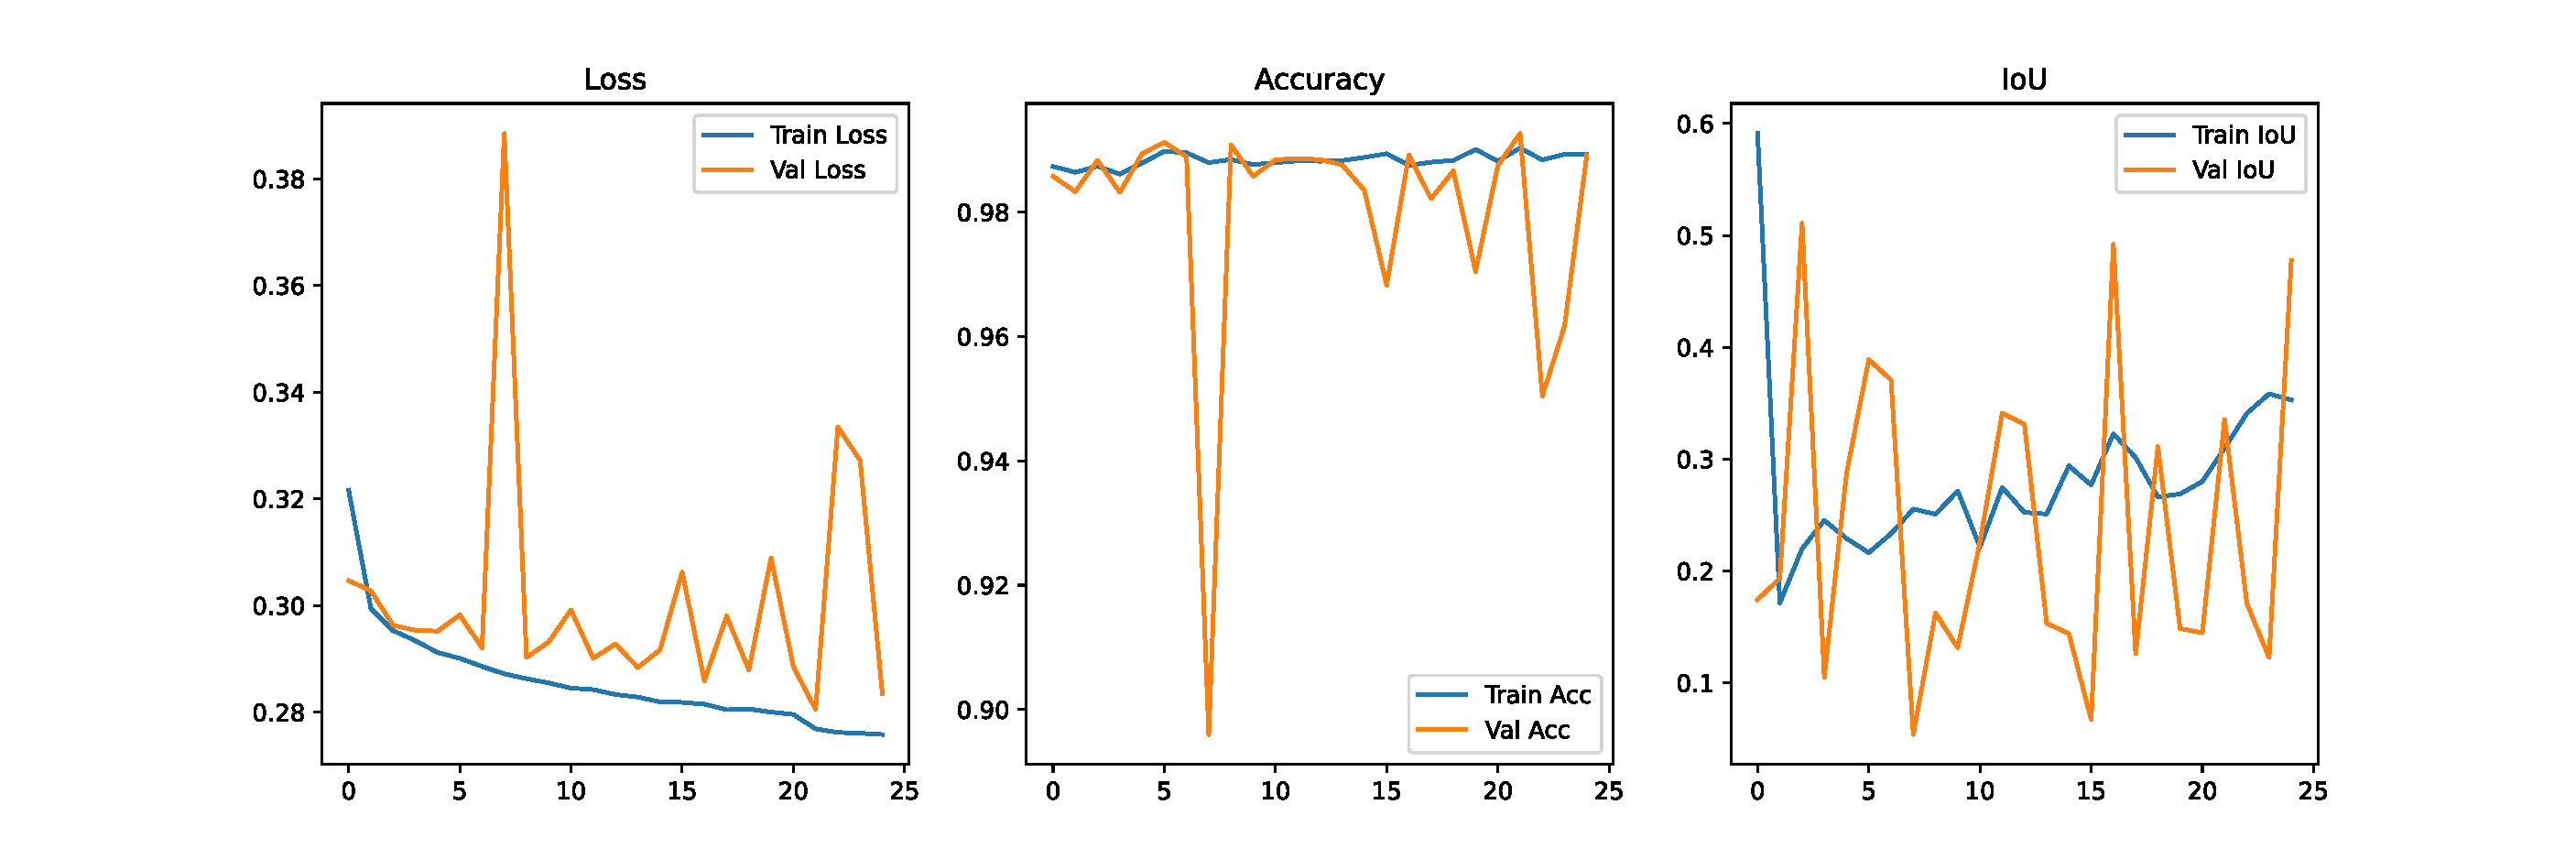
\includegraphics[width=0.8\textwidth]{plots/ures.pdf}
    \caption{Unet with ResNet34 Learning Curve}
    \label{fig:unet_res34}
\end{figure}

\begin{figure}[H]
    \centering
    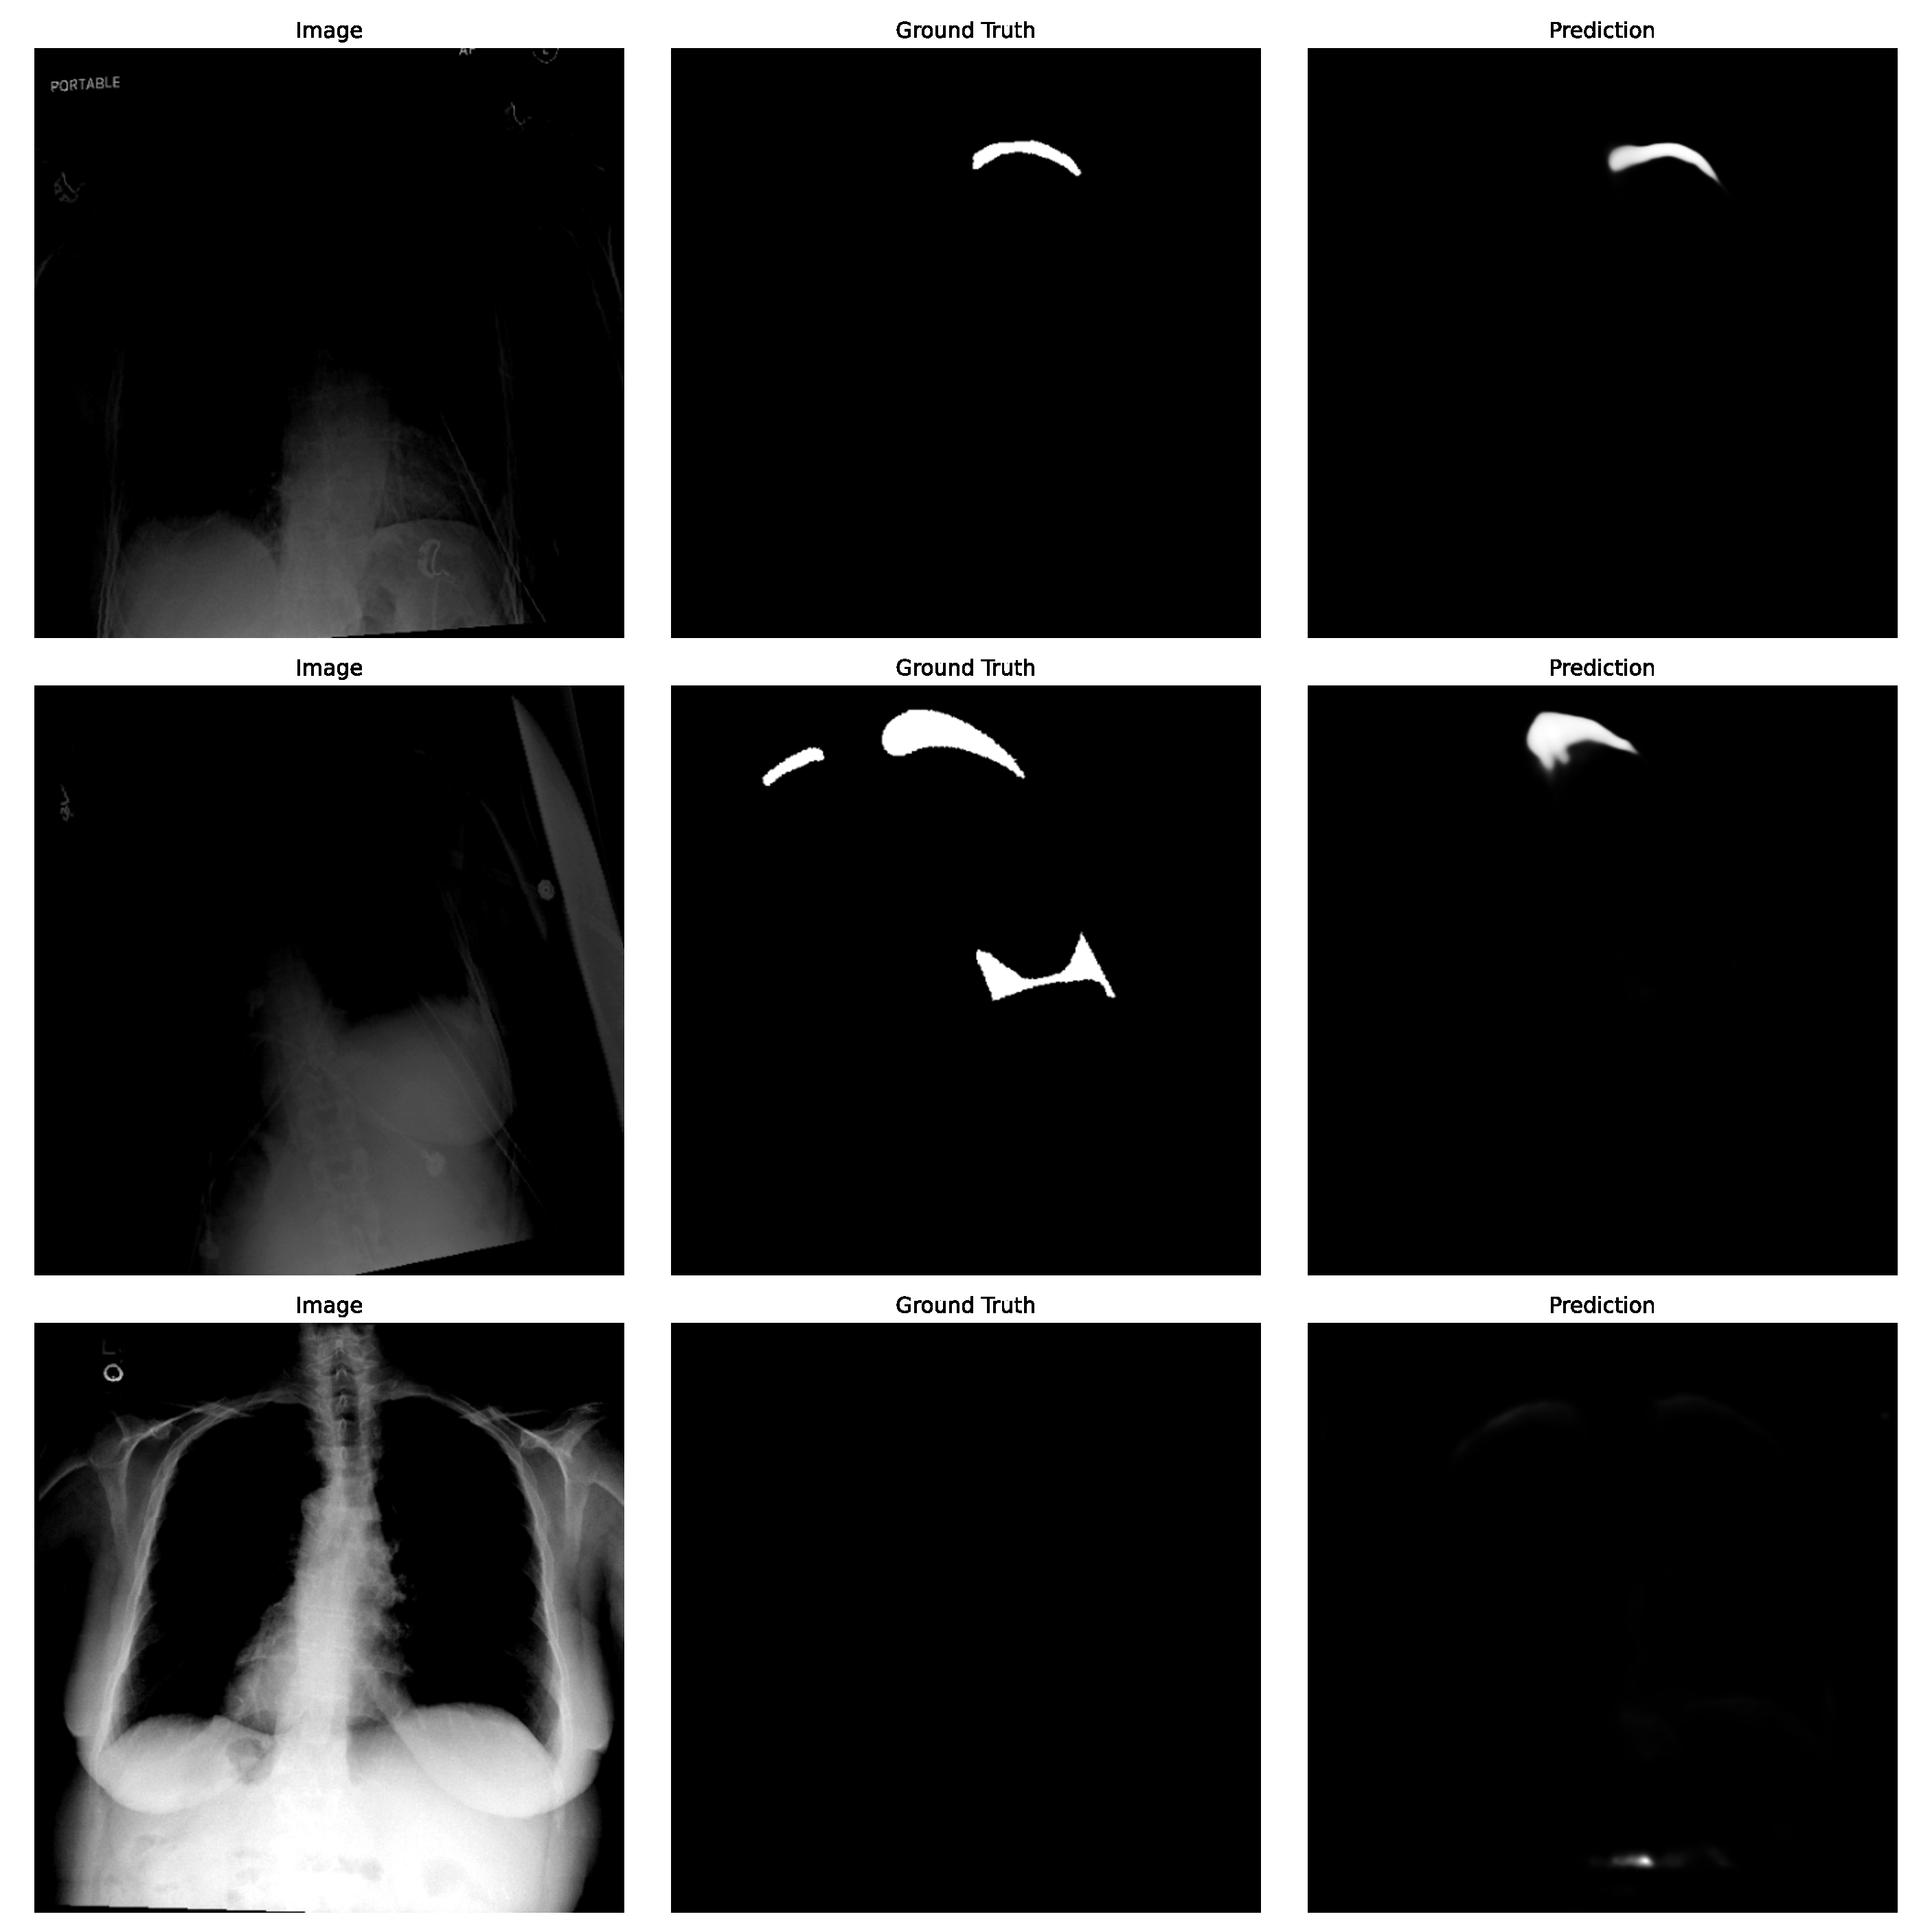
\includegraphics[width=0.8\textwidth]{plots/uresp.pdf}
    \caption{Unet with ResNet34 Example Predictions}
    \label{fig:unet_res34_p}
\end{figure}

\subsection*{Unet with VGG16}
Learning curves and example predictions are provided for U-Net with VGG16 backbone.

\begin{figure}[H]
    \centering
    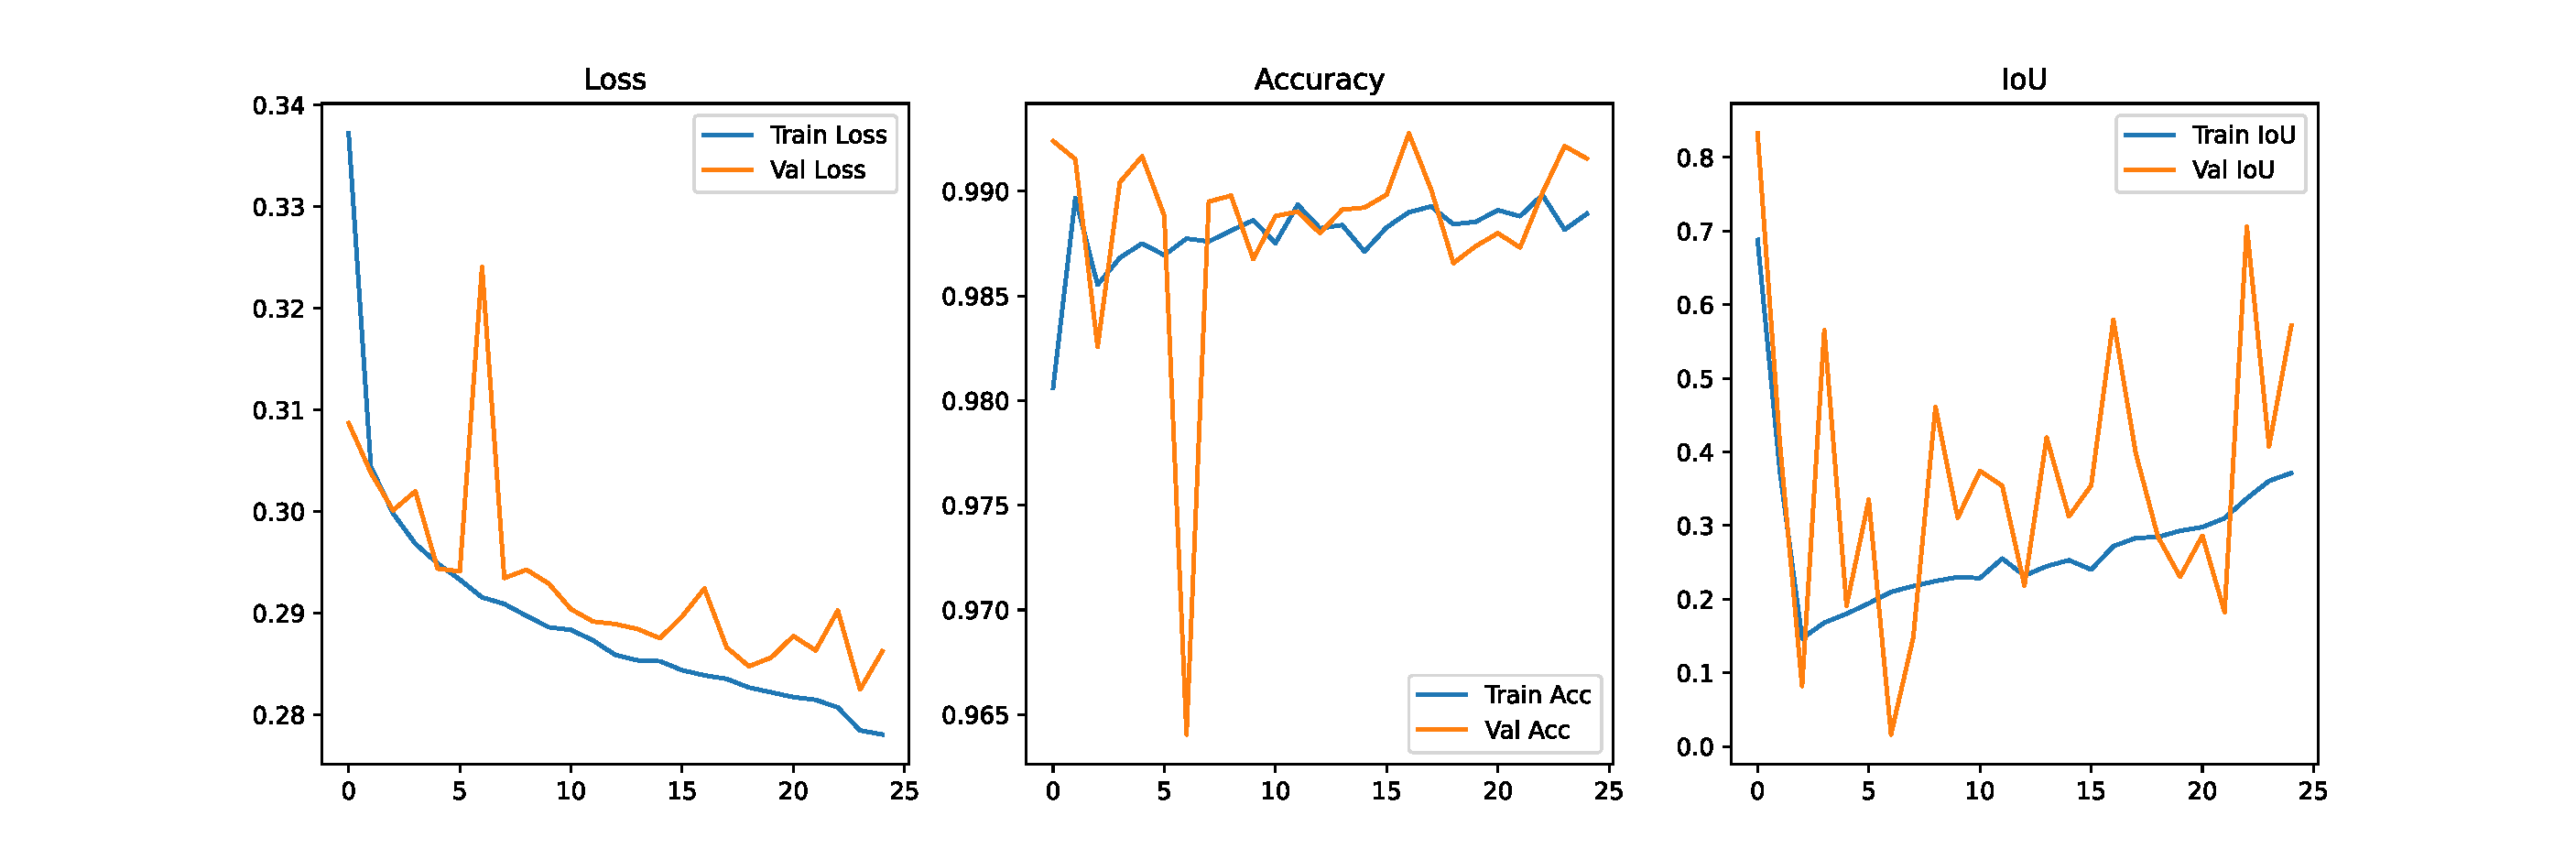
\includegraphics[width=0.8\textwidth]{plots/uvg.pdf}
    \caption{Unet with VGG16 Learning Curve}
    \label{fig:unet_vgg16}
\end{figure}

\begin{figure}[H]
    \centering
    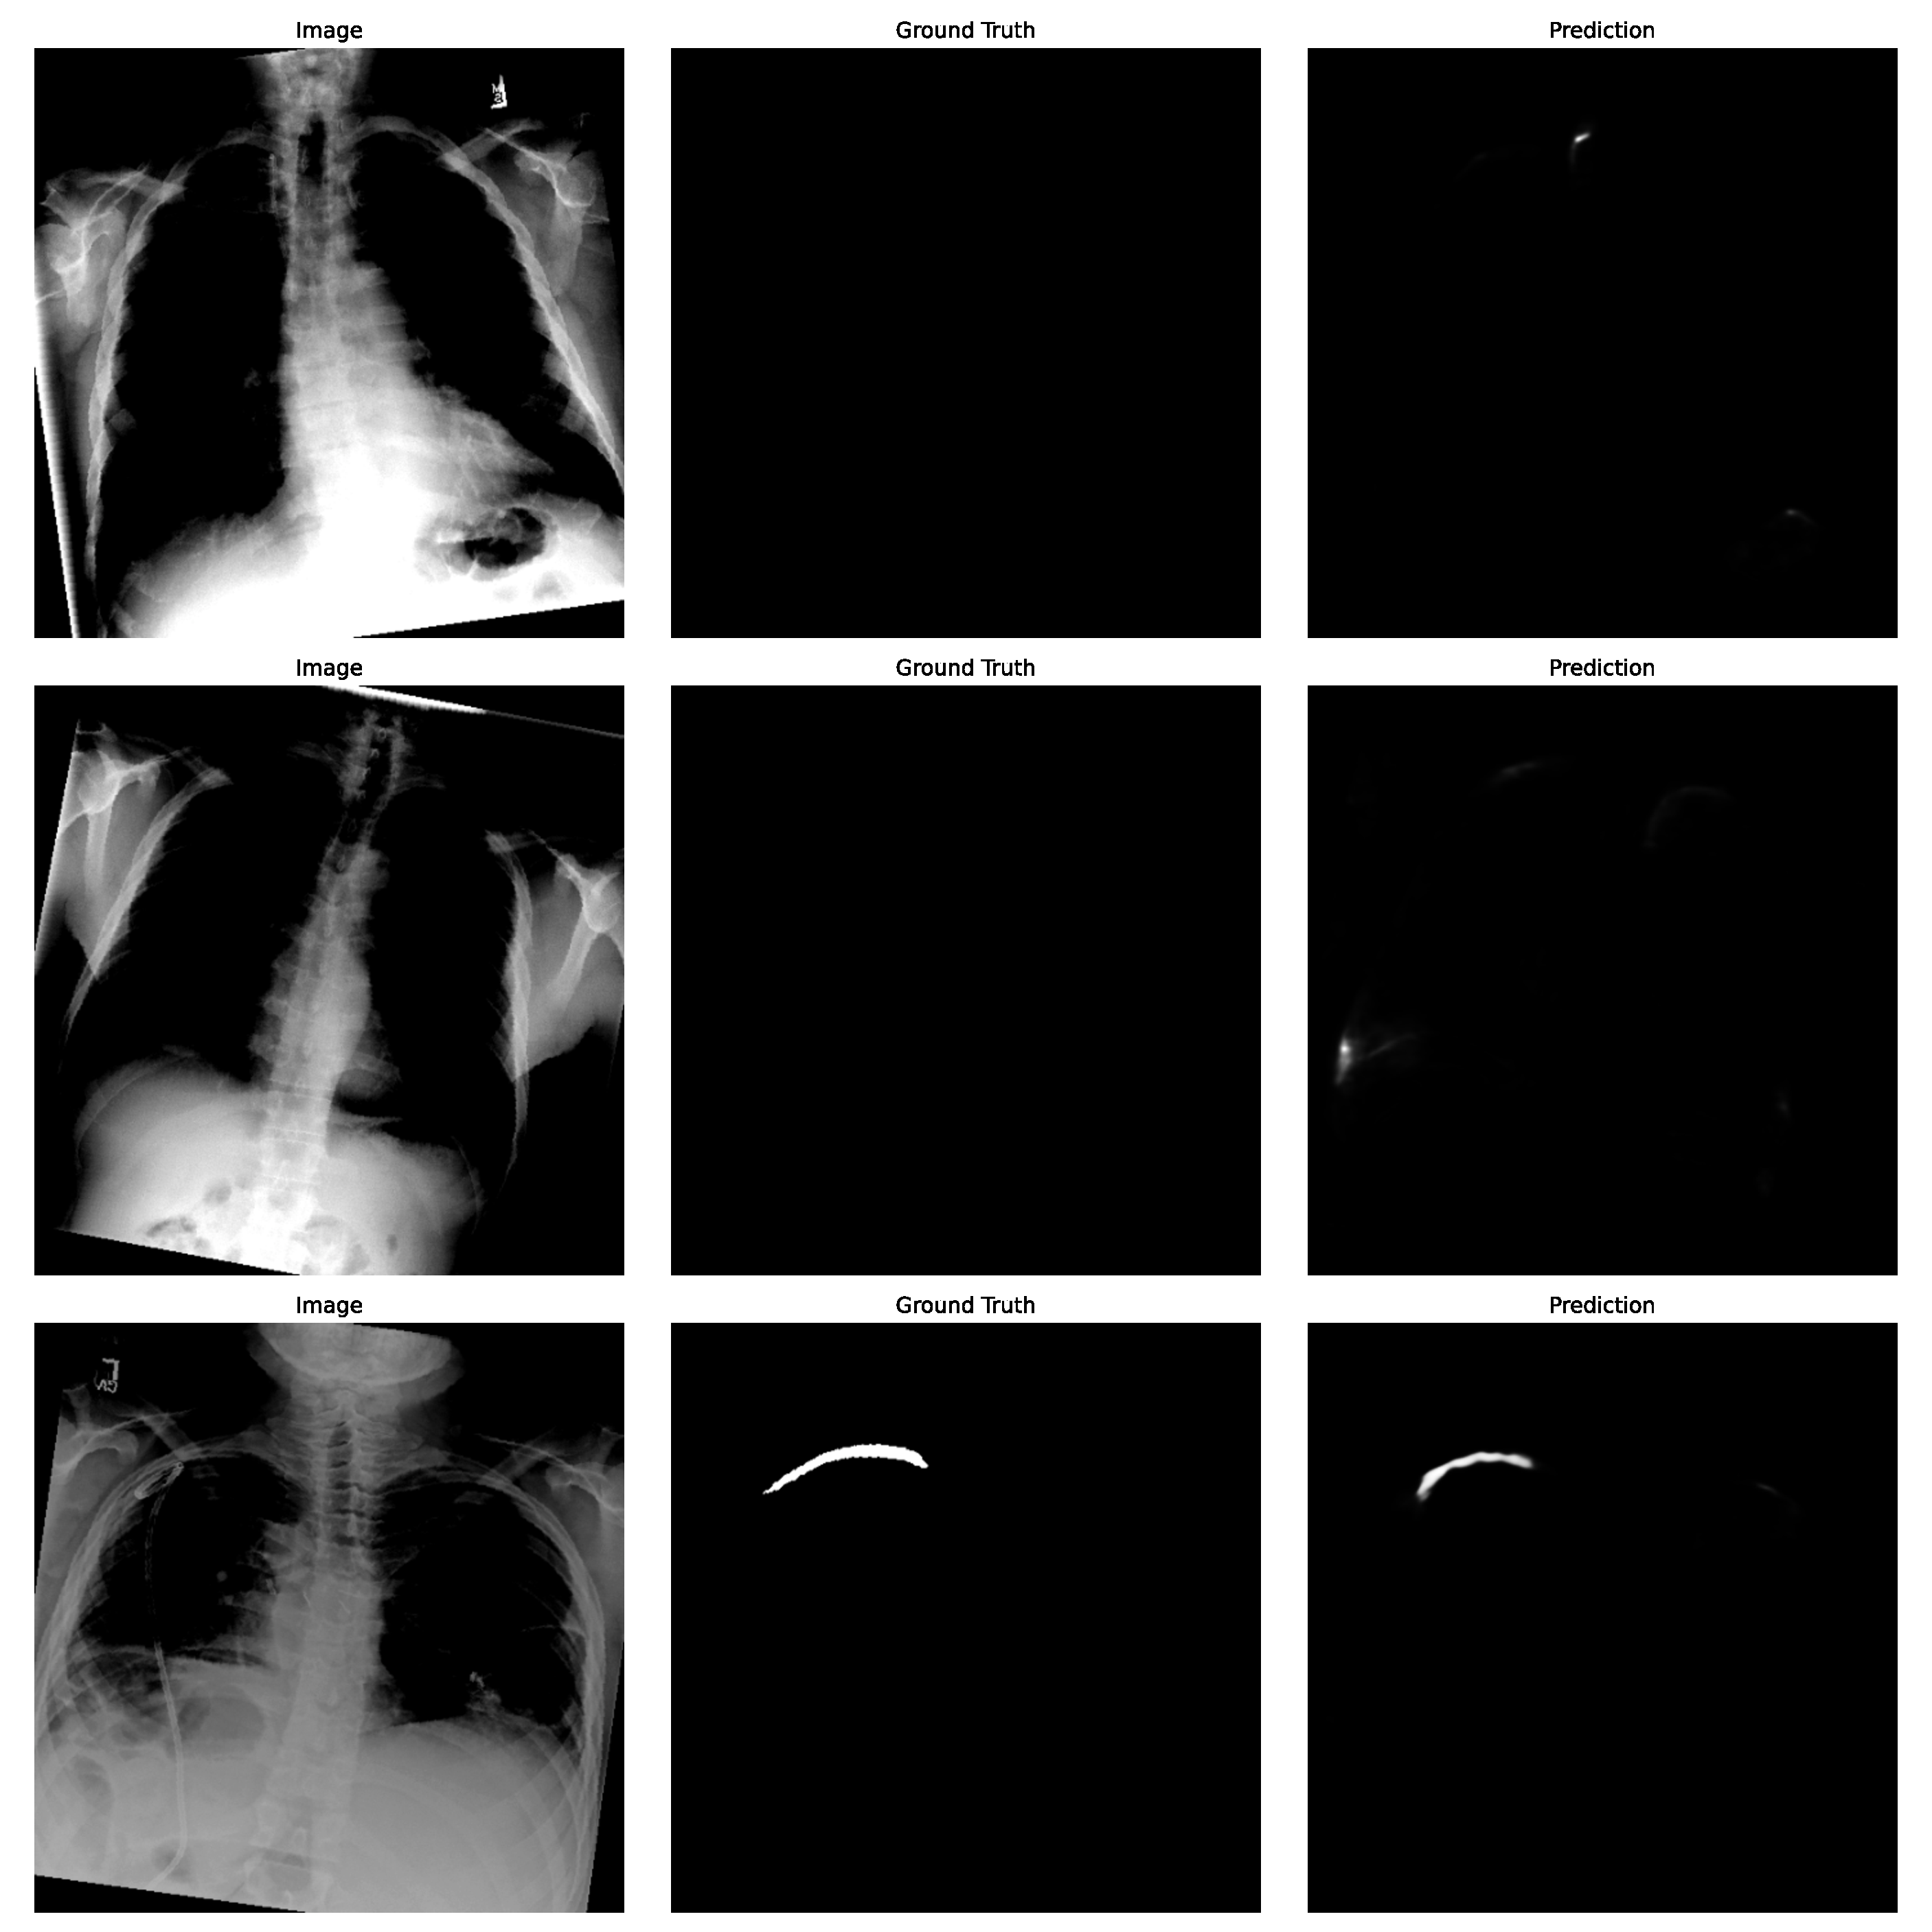
\includegraphics[width=0.8\textwidth]{plots/uvgp.pdf}
    \caption{Unet with VGG16 Example Predictions}
    \label{fig:unet_vgg16_p}
\end{figure}

\subsection*{Unet with InceptionResNetV2}
Learning curves and example predictions are provided for U-Net with InceptionResNetV2 backbone.

\begin{figure}[H]
    \centering
    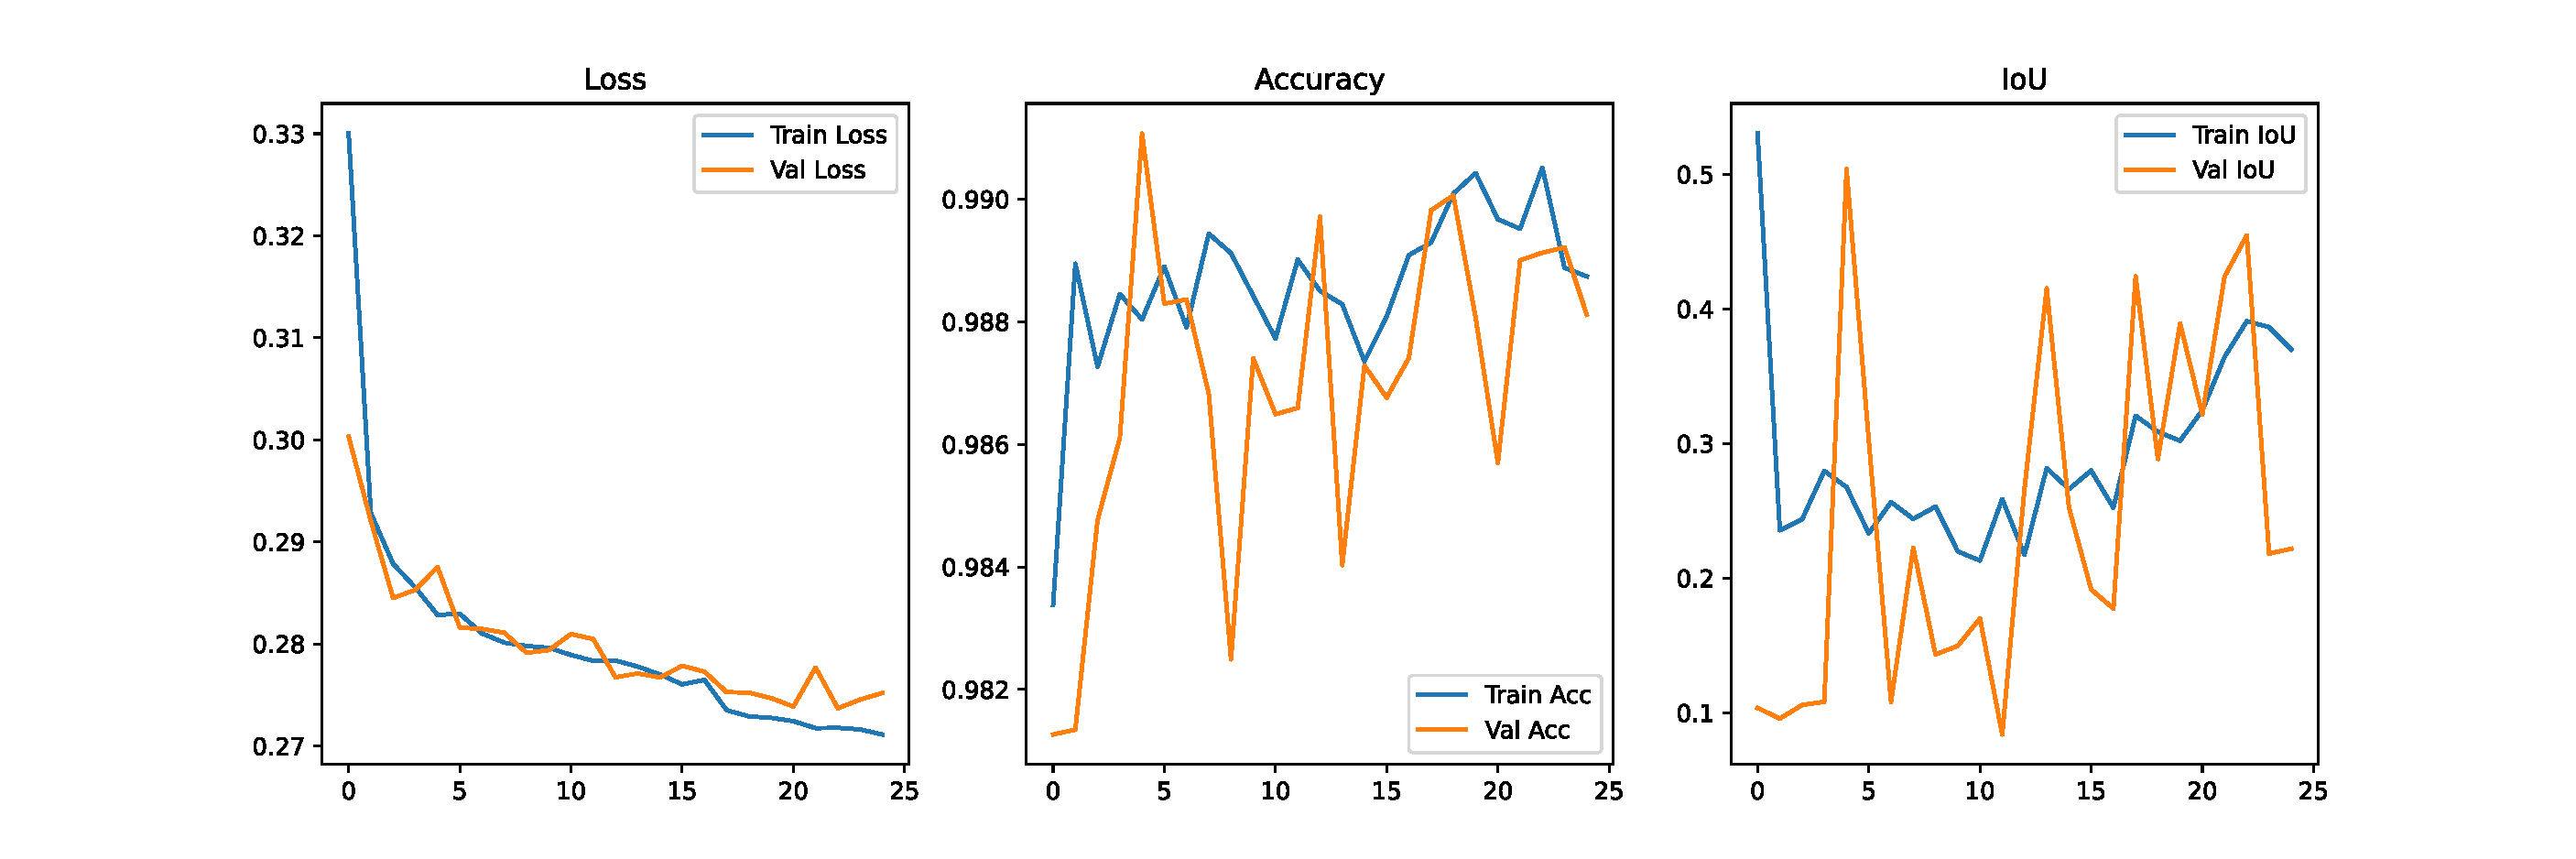
\includegraphics[width=0.8\textwidth]{plots/uinc.pdf}
    \caption{Unet with InceptionResNetV2 Learning Curve}
    \label{fig:unet_inception_resnetv2}
\end{figure}

\begin{figure}[H]
    \centering
    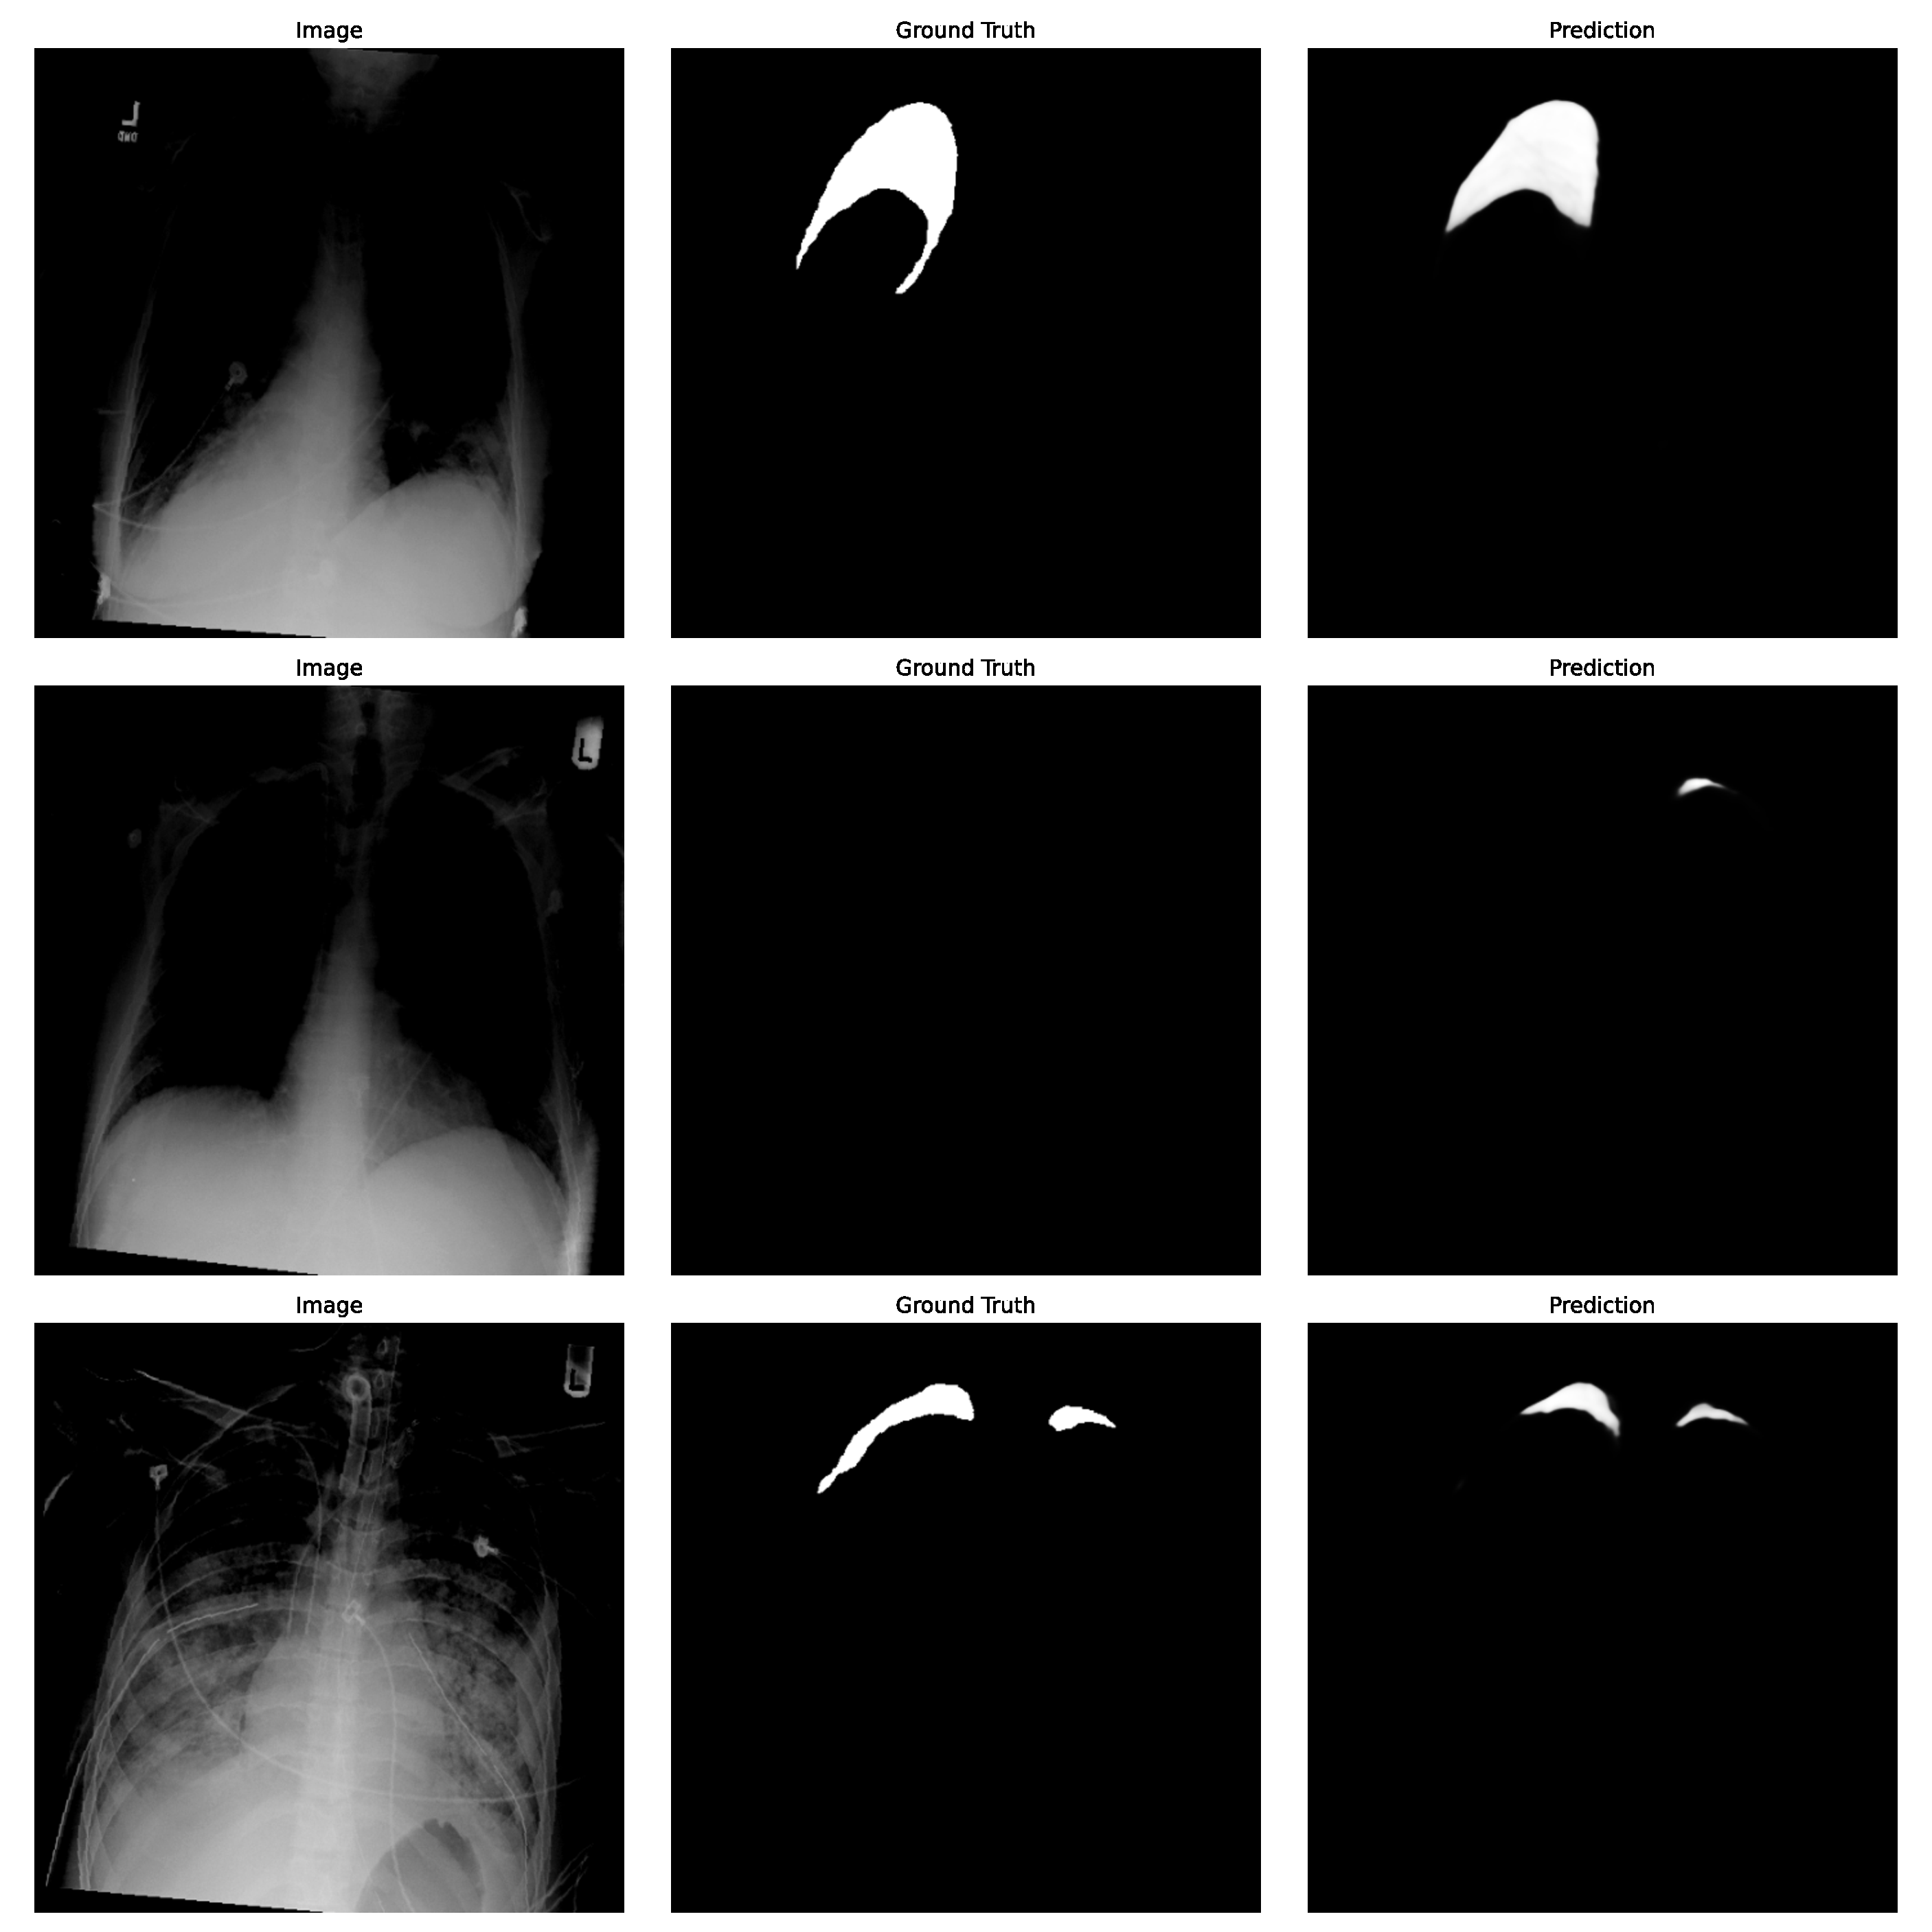
\includegraphics[width=0.8\textwidth]{plots/uincp.pdf}
    \caption{Unet with InceptionResNetV2 Example Predictions}
    \label{fig:unet_inception_resnetv2_p}
\end{figure}

\subsection*{Unet with Xception}
Learning curves and example predictions are provided for U-Net with Xception backbone.

\begin{figure}[H]
    \centering
    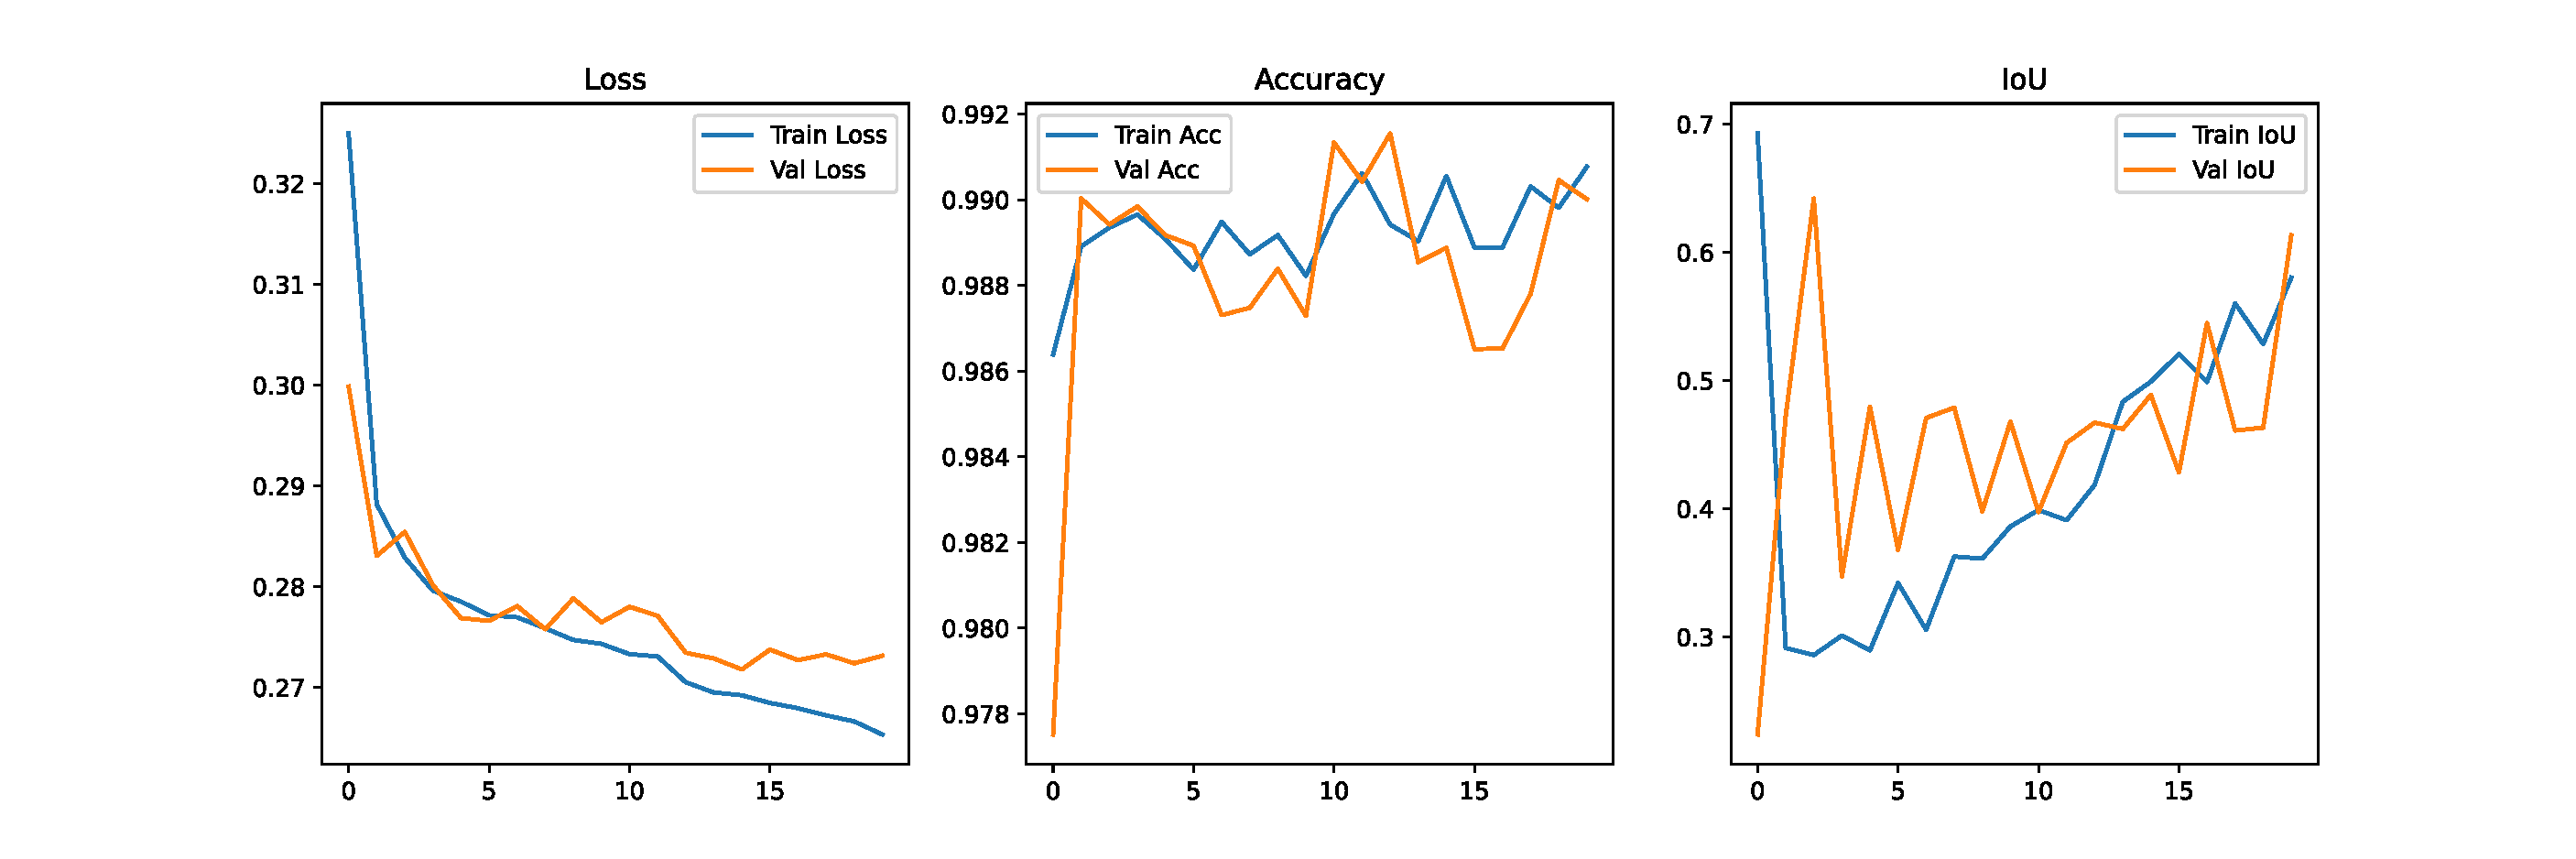
\includegraphics[width=0.8\textwidth]{plots/uxp.pdf}
    \caption{Unet with Xception Learning Curve}
    \label{fig:unet_xception}
\end{figure}

\begin{figure}[H]
    \centering
    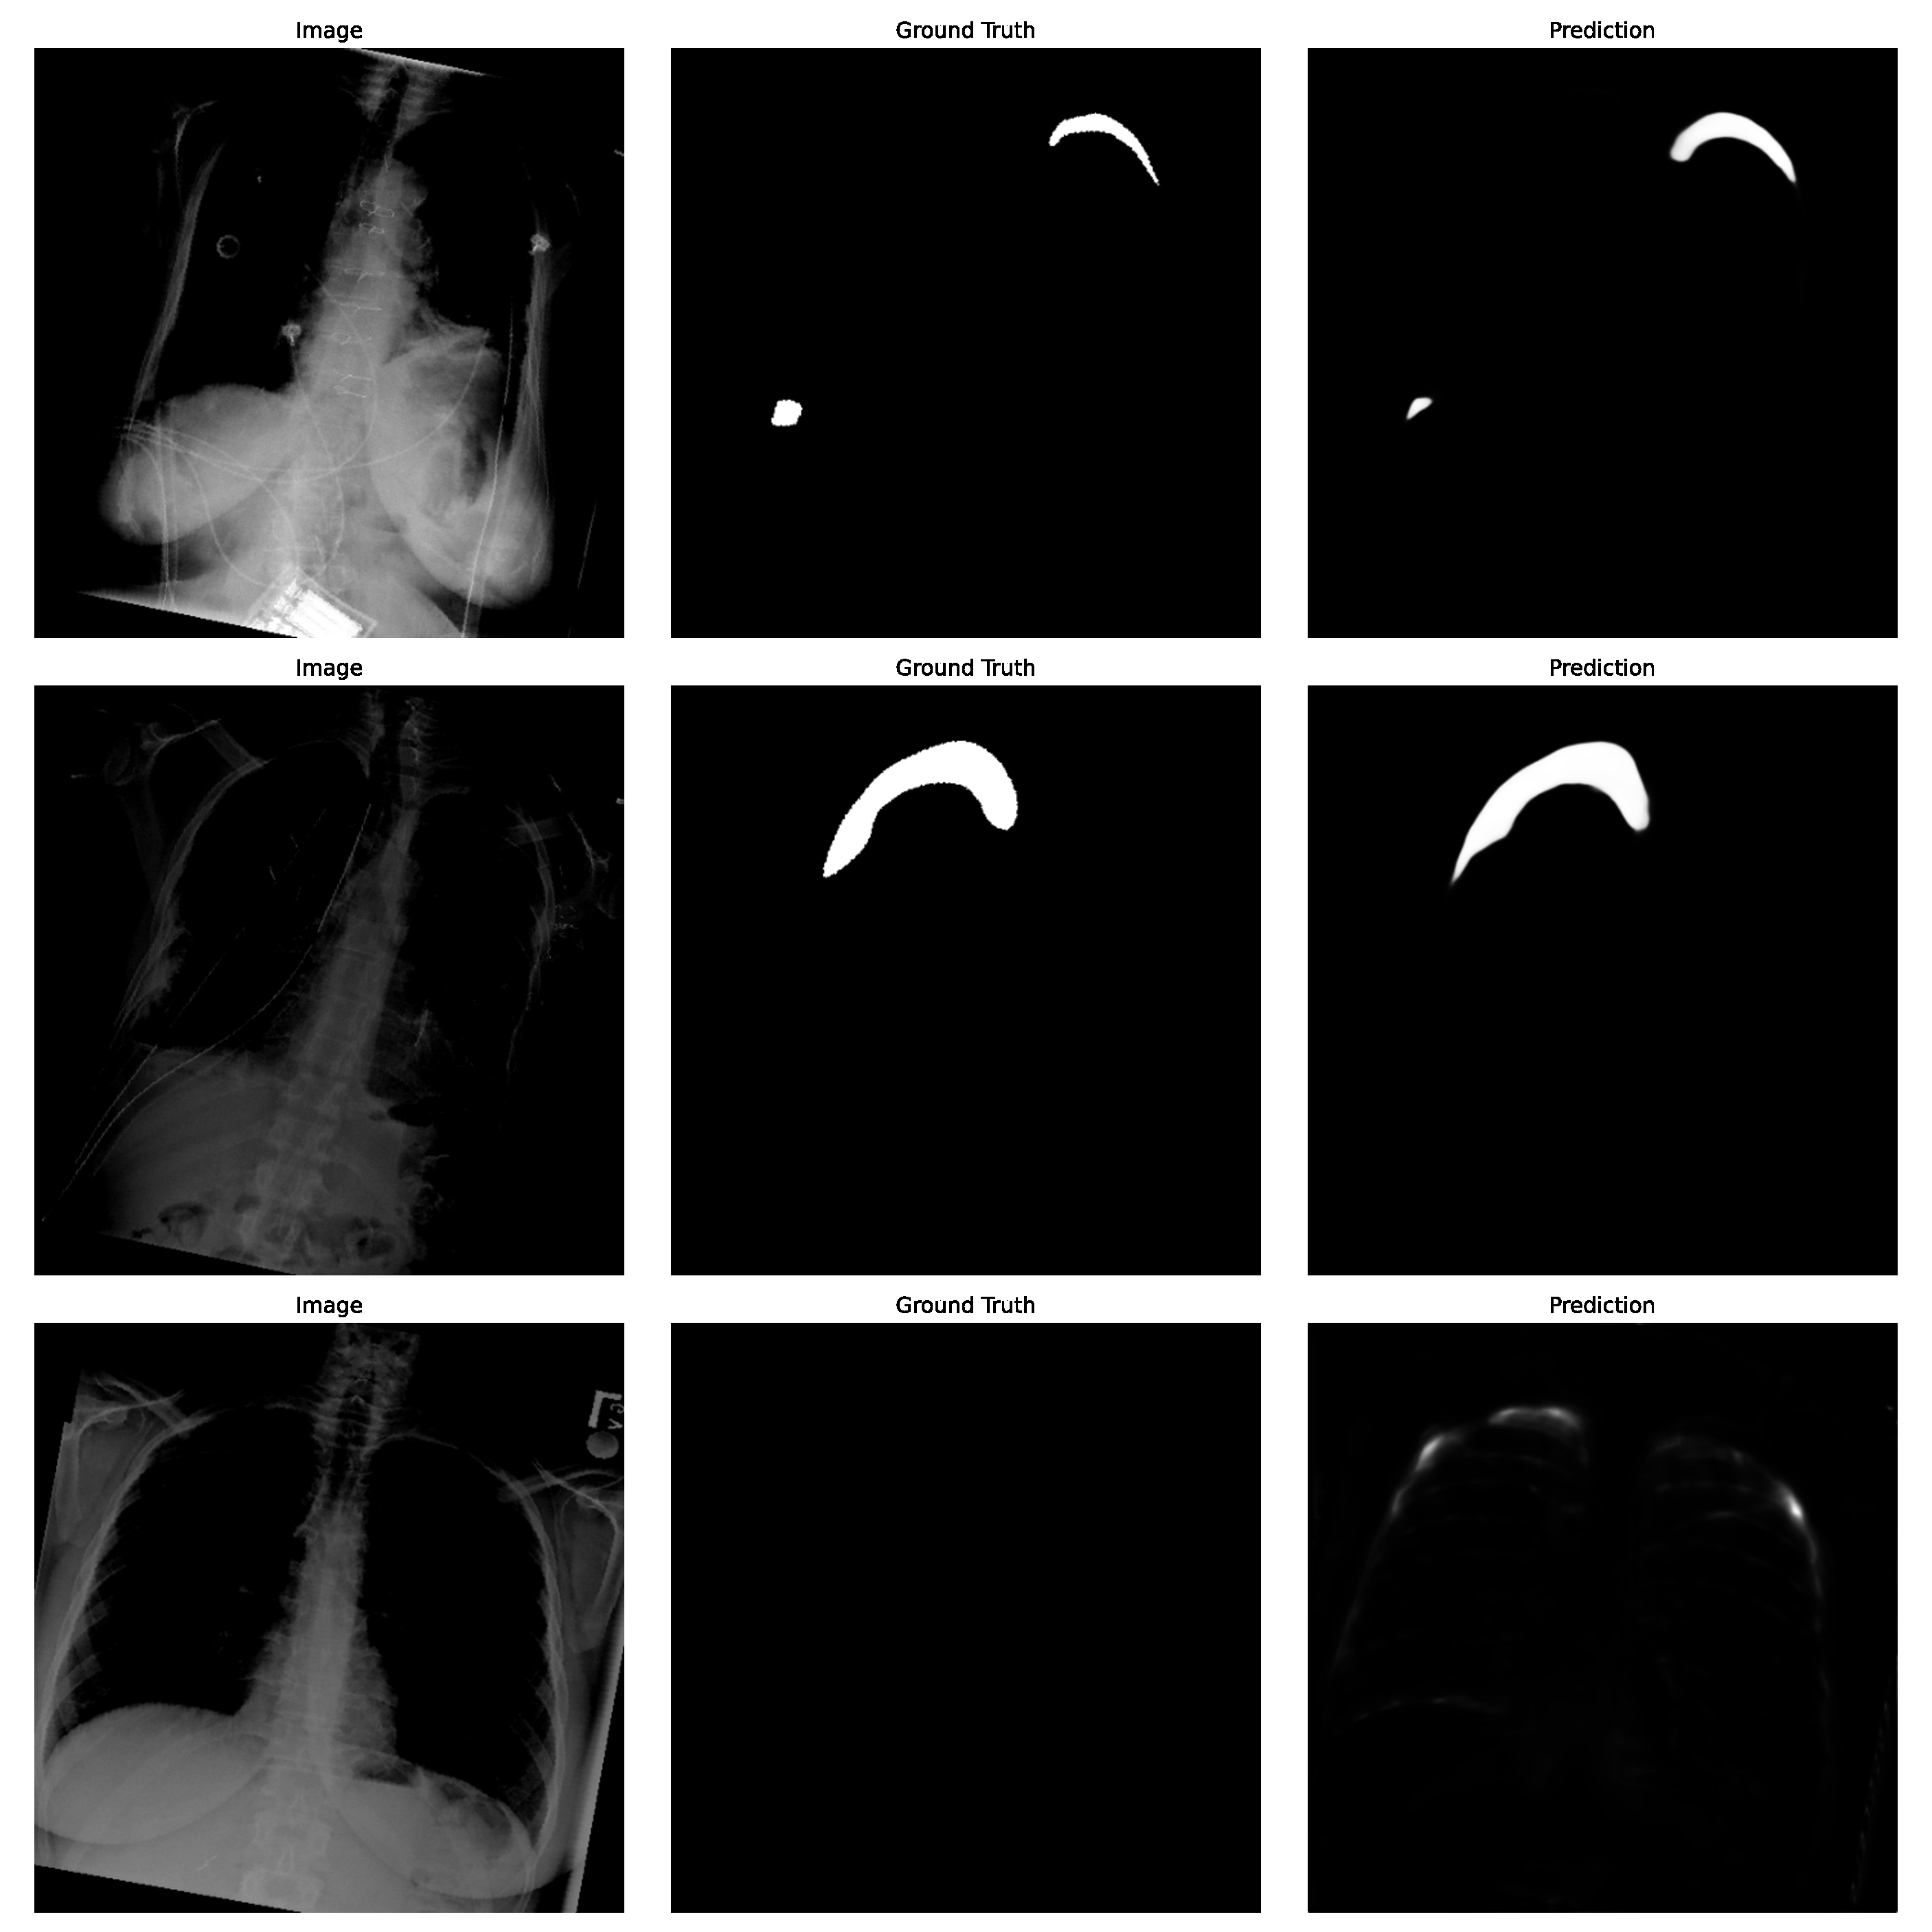
\includegraphics[width=0.8\textwidth]{plots/uxpp.pdf}
    \caption{Unet with Xception Example Predictions}
    \label{fig:unet_xception_p}
\end{figure}

\section*{Comparison}
\begin{tabular}{|l|c|c|c|}
\hline
\textbf{Model} & \textbf{Loss} & \textbf{IoU} & \textbf{Accuracy} \\
\hline
ResNet34 & 0.2761 & 0.4733 & 0.9885 \\
VGG16 & 0.2811 & 0.5504 & 0.9928 \\
InceptionResNetV2 & 0.2718 & 0.2238 & 0.9943 \\
Xception & 0.2674 & 0.6085 & 0.9920 \\
\hline
\end{tabular}

\section*{Final Thoughts on Segmentation Phase}
Based on the results, while InceptionResNetV2 achieved the highest accuracy, Xception stands out as the preferred choice for medical segmentation tasks due to its lower loss and superior mask prediction performance. Xception was also the fastest in terms of prediction time, making it efficient and reliable for this application.

\section*{Experimental Results for Classification}
For classification, Xception was used to predict the masks due to its superior performance compared to the other models.

\subsection*{Before Hyperparameter Tuning}
\begin{figure}[H]
    \centering
    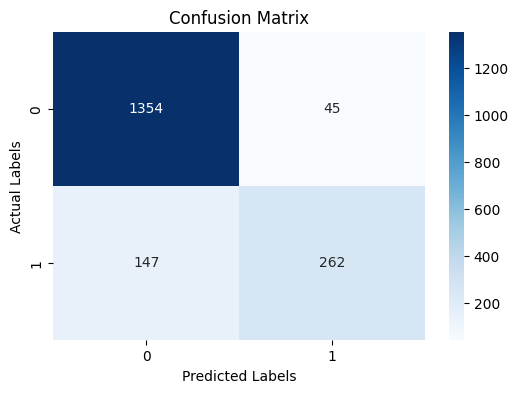
\includegraphics[width=0.8\textwidth]{plots/xgbconf_before.png}
    \caption{Confusion Matrix Before Hyperparameter Tuning}
    \label{fig:class_conf_before}
\end{figure}

\begin{figure}[H]
    \centering
    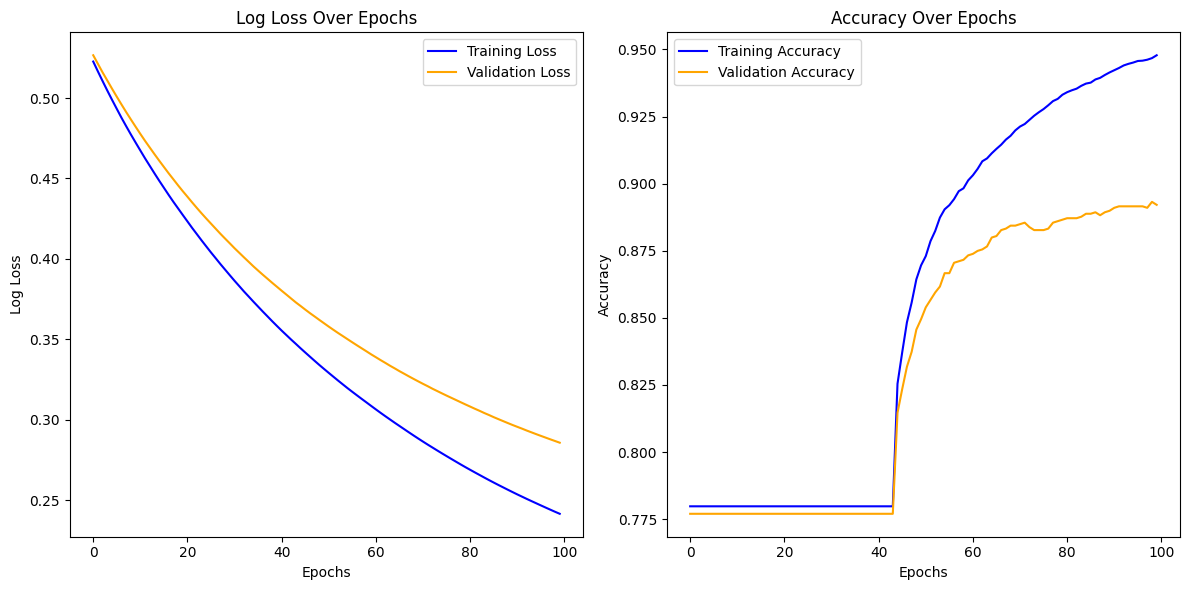
\includegraphics[width=0.8\textwidth]{plots/xgb_learning_before.png}
    \caption{Learning Curves Before Hyperparameter Tuning}
    \label{fig:class_learn_before}
\end{figure}


\subsection*{After Hyperparameter Tuning}
\begin{figure}[H]
    \centering
    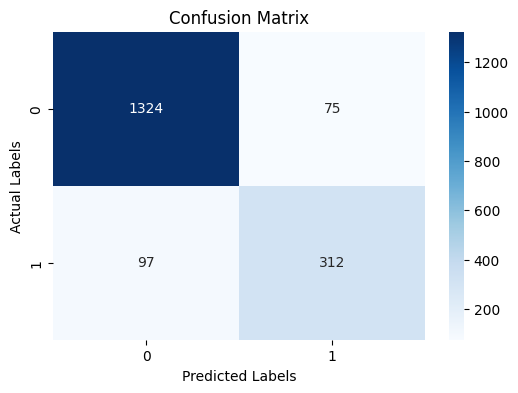
\includegraphics[width=0.8\textwidth]{plots/xgbconf_after.png}
    \caption{Confusion Matrix After Hyperparameter Tuning}
    \label{fig:class_conf_after}
\end{figure}
\begin{figure}[H]
    \centering
    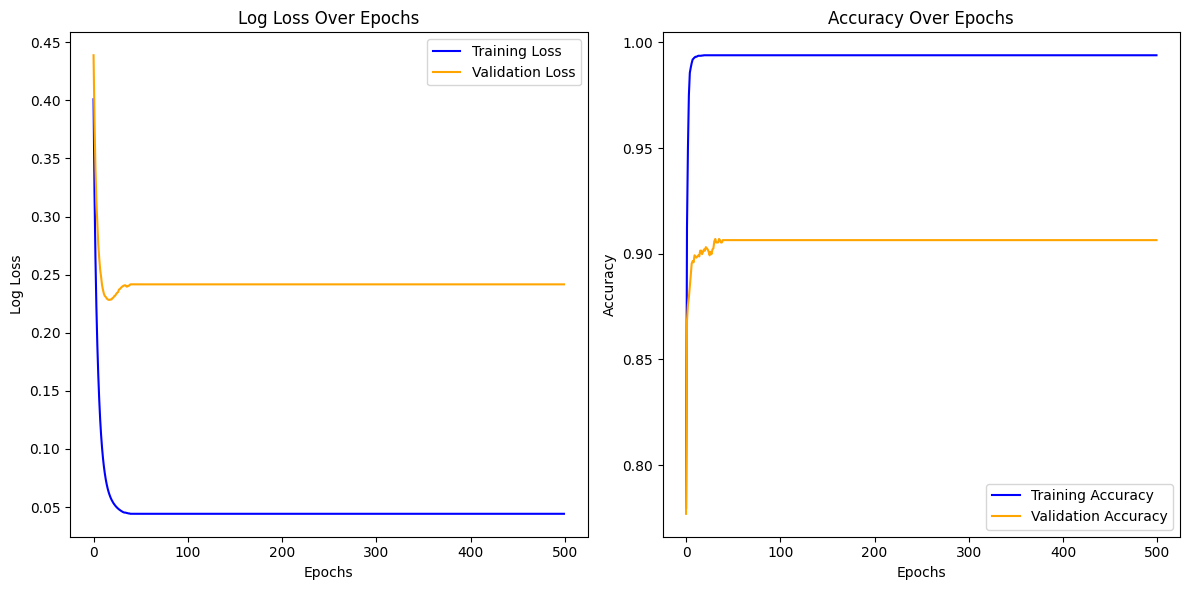
\includegraphics[width=0.8\textwidth]{plots/xgb_learning_after.png}
    \caption{Learning Curves After Hyperparameter Tuning}
    \label{fig:class_learn_after}
\end{figure}

\section*{Comparison}
\begin{tabular}{|l|c|c|c|c|}
\hline
\textbf{} & \textbf{Class} & \textbf{Precision} & \textbf{Recall} & \textbf{F1 Score} \\
\hline
Before Random Search & 0 & 0.90 & 0.97 & 0.93\\
 & 1 & 0.85 & 0.64 & 0.73\\
\hline
After Random Search & 0 & 0.93 & 0.95 & 0.94\\
 & 1 & 0.81 & 0.76 & 0.78\\
\hline
\end{tabular}


\section*{Final Thoughts on Classification Phase}
After conducting a random search with the XGBoost classifier, the model demonstrated a strong recall for detecting pneumothorax, especially in identifying positive cases. However, the learning curve shows overfitting, indicating limited generalization to new, unseen data. Exploring a deep learning-based classifier may offer a more robust solution, improving both recall and overall performance while mitigating overfitting issues.

\end{document}
